% !TeX program = xelatex
\documentclass[12pt, a4paper]{article}

% --- پکیج‌های پایه و ضروری ---
\usepackage[margin=2.5cm, headheight=14pt]{geometry}
\usepackage{amsmath, amssymb}
\usepackage{graphicx}
\usepackage{enumitem}
\usepackage{fancyhdr}
\usepackage{hyperref}
\usepackage{placeins}

% --- تنظیمات پیوند‌ها (لینک‌های سیاه) ---
\hypersetup{
	colorlinks=true,
	linkcolor=black,
	urlcolor=black
}

% --- پشتیبانی فارسی (ساده‌ترین و پایدارترین حالت) ---
% --- پشتیبانی فارسی ---
% --- پشتیبانی فارسی ---
% --- پشتیبانی فارسی ---
% --- پشتیبانی فارسی ---
% --- پشتیبانی فارسی ---
% --- پشتیبانی فارسی ---
% --- پشتیبانی فارسی ---
% --- پشتیبانی فارسی ---
\usepackage{xepersian}

% فونت Times New Roman: کلاسیک، رسمی و مناسب کتاب
\settextfont{Times New Roman}
\setdigitfont{Times New Roman}

% دستور کدهای درون‌متنی
\newcommand{\code}[1]{\lr{\texttt{#1}}}

% --- تنظیمات سربرگ و پاورقی ---
\pagestyle{fancy}
\fancyhf{}
\fancyhead[R]{\small گزارش فنی سامانه پیش‌بینی هوا}
\fancyfoot[C]{\thepage}
\renewcommand{\headrulewidth}{0.4pt}

\setlength{\parindent}{1.5cm}
\setlength{\parskip}{0.3em}

\begin{document}
	\thispagestyle{empty}
	\begin{titlepage}
		\centering
		
		% اگر عکس لوگو را ندارید، کلمه demo را داخل براکت بنویسید: 
\includegraphics[demo, width=0.24\textwidth]{logo.png}
		
\includegraphics[width=0.24\textwidth]{logo.png}
		
		\vspace{1.8cm}
		
		{\large\bfseries دانشکده علوم ریاضی}\\[0.25cm]
		{\large گروه آمار}
		
		\vspace{1.8cm}
		
		{\huge\bfseries سامانه پیش‌بینی آب و هوا}\\[0.35cm]
		{\large\bfseries \lr{WFS Dashboard}}
		\vspace{0.5cm}
		
		\begin{minipage}{0.82\textwidth}
			\centering
			{\large
				ارزیابی و مقایسه مدل‌های یادگیری ماشین و آماری\\
				در پیش‌بینی سری‌های زمانی هواشناسی
			}
		\end{minipage}
		
		\vspace{2cm}
		
		\begin{tabular}{c}
			{\large\bfseries توسعه‌دهنده}\\[0.25cm]
			{\large مهدیه ابراهیمی}\\[0.9cm]
			
			{\large\bfseries استاد راهنما}\\[0.25cm]
			{\large دکتر محمد آرشی}
		\end{tabular}
		
		\vfill
		
		{\large نیمسال دوم سال تحصیلی ۱۴۰۴-۱۴۰۵}
		
		\vspace{0.7cm}
		
	\end{titlepage}
	\newpage
	
	% --- فهرست مطالب ---
	\thispagestyle{empty}
	{\small 
		\tableofcontents
	}
	\newpage
	
	% ==========================================================
	\section{مقدمه و صورت مسئله}
	% ==========================================================
	
	\subsection{زمینه و انگیزه پژوهش}
	توسعه مدل‌های پیش‌بینی هوا به طور سنتی در انحصار مدل‌های عددی پیش‌بینی هوا \lr{(NWP)} بود که با حل معادلات دیفرانسیل پیچیده جو کار می‌کنند. با ظهور یادگیری ماشین، این پرسش علمی مطرح شد که "آیا مدل‌های داده‌محور \lr{(Data-Driven)} می‌توانند با تکیه صرفاً بر داده‌های تاریخی و الگوهای آماری، جایگزین یا رقیب مدل‌های فیزیکی شوند؟"
	هدف اصلی این پژوهش، نه صرفاً ساخت یک ابزار پیش‌بینی، بلکه \textbf{مقایسه و ارتقای مدل‌های هوش مصنوعی و آماری} است تا مشخص شود حداکثر دقت قابل دستیابی بدون دخالت مدل‌های \lr{NWP} چقدر است و سیستم در کدام بخش‌ها و افق‌های زمانی دچار ناتوانی می‌شود.
	
	\subsection{صورت مسئله و چالش‌های مدل‌های داده‌محور}
	مسئله ما، پیش‌بینی متغیرهای جوی (مانند دما) برای ۵ کلان‌شهر ایران در دو افق کوتاه‌مدت (۲۴ ساعته) و میان‌مدت (۷ روزه) با استفاده از ۱۱ مدل مختلف است.
	در مسیر ارتقای این مدل‌ها، متوجه شدیم که تکیه صرف بر الگوریتم‌های یادگیری ماشین (مانند \code{XGBoost} یا \code{LightGBM}) در غیاب فیزیک اتمسفری، با چالش‌های بنیادین روبرو است:
	
	\begin{enumerate}[label=\arabic*.]
		\item \textbf{سقف دقت در کوتاه‌مدت:} مدل‌های \lr{ML} به دلیل درک هم‌خطی بین متغیرهای تاخیری \lr{(Lags)}، در افق ۲۴ ساعت عملکرد فوق‌العاده‌ای دارند و می‌توانند با \lr{NWP} رقابت کنند.
		\item \textbf{فروپاشی در افق دور (جایی که به \lr{NWP} نیاز داریم):} به محض عبور از افق ۴۸ ساعت، مدل‌های درختی به دلیل عدم توانایی در برون‌یابی روند \lr{(Extrapolation)} و انباشت خطا در پیش‌بینی بازگشتی، دچار سقوط شدید دقت می‌شوند و خطوط پیش‌بینی آن‌ها به سمت مقادیر ثابت یا غیرفیزیکی میل می‌کند \lr{(Flat-line Collapse)}.
	\end{enumerate}
	
	\subsection{رویکرد سیستم: ارتقا تا مرز فیزیک}
	برای پاسخ به این چالش‌ها و کشف مرزهای مدل‌های داده‌محور، ما یک معماری چندلایه طراحی کردیم:
	\begin{itemize}
		\item \textbf{ارتقای الگوریتم‌های \lr{ML}:} برای جلوگیری از فروپاشی مدل‌ها در ۷ روز آینده، استراتژی پیش‌بینی بازگشتی به \textbf{\lr{Direct Multi-Horizon}} (مدل‌سازی مستقل برای هر روز) تغییر یافت. همچنین از تکنیک \textbf{\lr{Anomaly Targeting}} (پیش‌بینی انحراف از میانگین اقلیمی) استفاده شد تا بارِ یادگیری فیزیک فصل‌ها از دوش مدل برداشته شود.
		\item \textbf{ترکیب نهایی با \lr{NWP} \lr{(MOS Blending)}:} پس از اعمال تمامی روش‌های ارتقای \lr{ML}، پذیرفتیم که مدل‌های داده‌محور در افق‌های میان‌مدت به سقف خود می‌رسند. به همین دلیل، \lr{Open-Meteo} (به عنوان نماینده مدل \lr{NWP}) را نه به عنوان رقیب، بلکه به عنوان یک ویژگی \lr{(Feature)} با خروجی \lr{ML} خودمان ترکیب کردیم \lr{(MOS Blending)}.
		\vspace{5cm}
	\end{itemize}
	
	% ==========================================================
	\section{نمای کلی سامانه}
	پیش از ورود به جزئیات فنی، این بخش یک نمای کلی از رابط کامل داشبورد پیاده‌سازی‌شده ارائه می‌دهد: صفحه اصلی، منوی ناوبری کناری با ۶ بخش، و آمار واقعی ثبت‌شده برای هر شهر.
	
	\vspace{1cm}
	\begin{figure}[htbp]
		\centering
		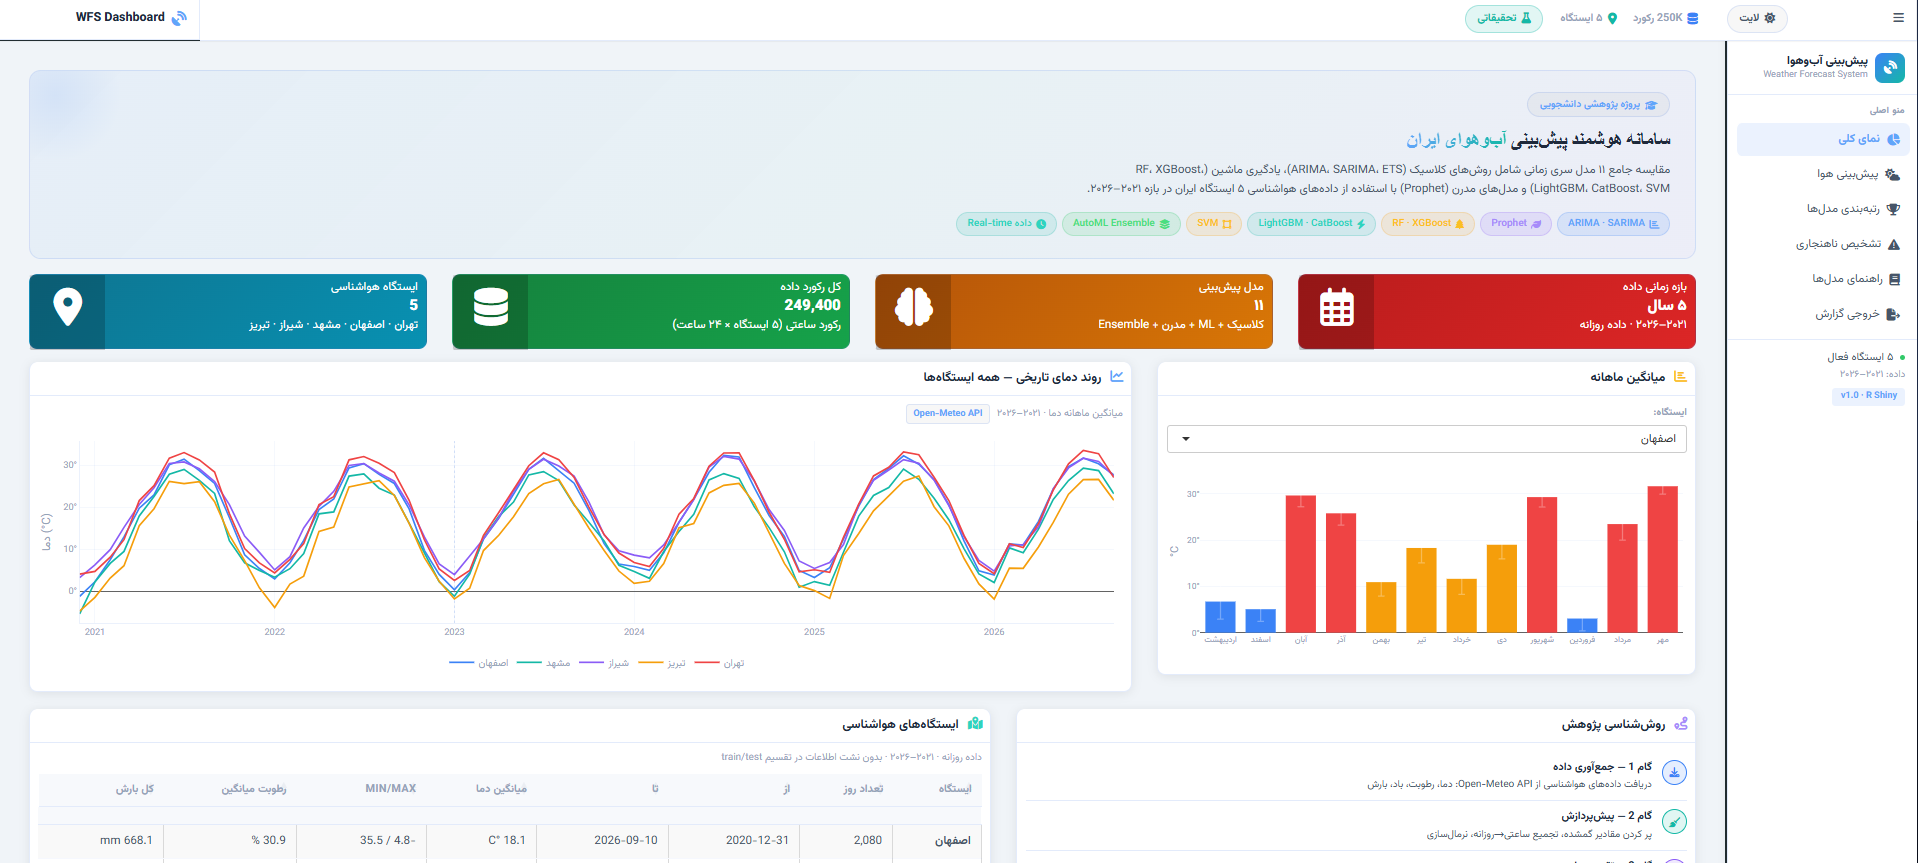
\includegraphics[width=0.95\linewidth]{figs/app_overview.png}
		\caption{نمای کلی اپلیکیشن که نمایش‌دهنده بخش‌های مختلف سامانه است.}
		\vspace{1cm}
	\end{figure}
	
	\begin{figure}[htbp]
		\centering
		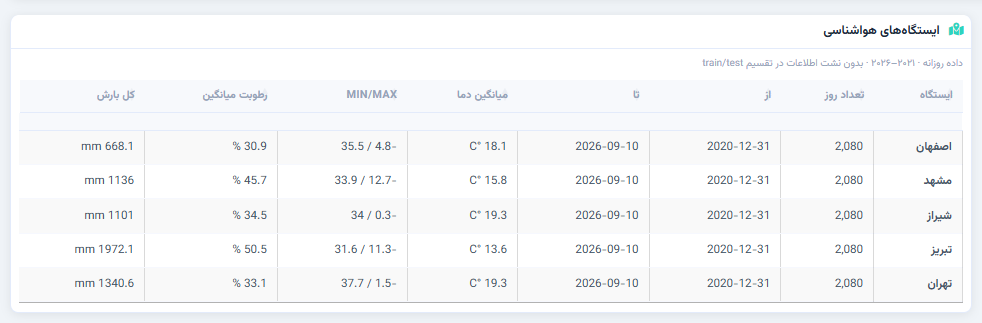
\includegraphics[width=0.95\linewidth]{figs/stations_table.png}
		\caption{آمار واقعی ۵ ایستگاه هواشناسی سامانه.}
		\vspace{2cm}
	\end{figure}
	\FloatBarrier
	
	\noindent کد منبع و فایل‌های اجرایی این سامانه به صورت متن‌باز در مخزن گیت‌هاب پروژه در دسترس عموم قرار گرفته است: 
	\begin{flushleft}
		\large \lr{\url{https://github.com/ebrahimyMahdiyeh/Shiny_weather_app}}
	\end{flushleft}
	\normalsize
	\FloatBarrier
	
	% ==========================================================
	\section{الزامات سیستم \lr{(System Requirements)}}
	% ==========================================================
	برای اجرای پایدار خط‌لوله مقایسه و ارتقای مدل‌ها، سیستم باید الزامات سخت‌گیرانه‌ای را در دو سطح عملکردی و غیرعملکردی برآورده سازد.
	
	\begin{figure}[htbp]
		\centering
		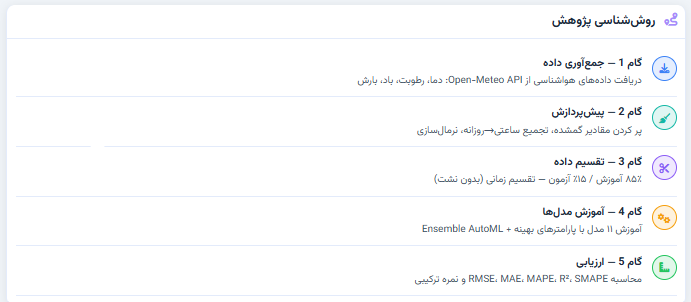
\includegraphics[width=0.6\linewidth]{figs/methodology_steps.png}
		\caption{روش‌شناسی پژوهش در ۵ گام.}
	\end{figure}
	\FloatBarrier
	
	\subsection{الزامات عملکردی \lr{(Functional Requirements)}}
	\begin{itemize}
		\item \textbf{دریافت و همگون‌سازی داده:} فراخوانی هم‌زمان دو \lr{End-point} آرشیو و پیش‌بینی \lr{Open-Meteo}.
		\item \textbf{بازسازی پیوستگی زمانی:} ساخت یک توری زمانی ساعتی کامل و بدون حفره.
		\item \textbf{مهندسی ویژگی:} محاسبه لگ‌های ۱ تا ۷۲ ساعته و رمزگذاری سینوسی-کوسینوسی چرخه‌های زمانی.
		\item \textbf{پشتیبانی چندگانه از افق پیش‌بینی:} روش بازگشتی برای افق ۲۴ ساعته و روش مستقیم برای افق ۷ روزه.
	\end{itemize}
	
	\subsection{الزامات غیرعملکردی \lr{(Non-Functional Requirements)}}
	\begin{itemize}
		\item \textbf{تضمین عدم نشت داده:} تقسیم داده کاملاً زمانی و متوالی.
		\item \textbf{مدیریت حافظه و کارایی:} استفاده از ساختارهای ماتریسی بهینه.
		\item \textbf{پایداری در برابر خطا:} احاطه تمام فراخوانی‌های مدل با مدیریت خطا.
		\item \textbf{قیود فیزیکی و اصلاح نویز:} حذف داده پرت با تکنیک \lr{IQR} ماهانه.
	\end{itemize}
	
	% ==========================================================
	\section{مدل داده و مهندسی ویژگی}
	% ==========================================================
	یکی از چالش‌های اصلی در استفاده از مدل‌های یادگیری ماشین، درک مفاهیم فیزیکی توسط این مدل‌هاست. 
	
	\subsection{پاک‌سازی پیشرفته و حذف نویز}
	داده‌های خام هواشناسی معمولاً حاوی نویزهای ناشی از خطای سنسورها هستند.
	\begin{itemize}
		\item \textbf{درون‌یابی خطی:} برای گپ‌های کوچک زمانی، سیستم از \code{zoo::na.approx} استفاده می‌کند.
		\item \textbf{حذف داده‌های پرت با \lr{IQR} ماهانه:} سیستم به صورت پویا، داده‌ها را بر اساس «ماه» گروه‌بندی کرده و بازه بین چارک اول و سوم را محاسبه می‌کند. هر دمایی که از بازه $[Q1 - 1.5 \times IQR, Q3 + 1.5 \times IQR]$ خارج باشد، به عنوان نویز شناسایی می‌شود.
	\end{itemize}
	
	\subsection{قیود فیزیکی و شاخص‌های اقلیمی}
	برای کمک به مدل‌های درختی تا منطق فیزیکی جو را درک کنند، ویژگی‌های جدیدی ساخته شدند:
	\begin{itemize}
		\item \textbf{قید منطقی ($T_{min} \leq T_{max}$):} سیستم پس از پیش‌بینی مقادیر بیشینه و کمینه، یک لایه ایمنی ریاضی اعمال می‌کند.
		\item \textbf{تقریب تابش خورشید (\code{solar\_rad}):} شدت تابش خورشید را با فرمول مثلثاتی مدل کردیم:
		\begin{equation}
			\theta = \sin\left(2\pi \frac{H - 6}{24}\right)
		\end{equation}
		که در آن $H$ ساعت روز است. مقادیر منفی صفر در نظر گرفته شده و در یک ضریب تصحیح فصلی $\left(1 + \cos\left(\frac{2\pi (D - 172)}{365}\right)\right)$ ضرب می‌شوند.
	\end{itemize}
	
	\subsection{ریاضیات متغیرها و رمزگذاری زمانی}
	زمان یک متغیر چرخه‌ای است. مثلاً ساعت ۲۳ بسیار به ساعت ۰۰ نزدیک‌تر است تا به ساعت ۱۲.
	\begin{itemize}
		\item \textbf{رمزگذاری سینوسی-کوسینوسی:} سیستم برای حفظ پیوستگی ریاضی حلقه‌های زمانی، ساعت و روز سال را به مختصات دکارتی تبدیل می‌کند:
		\begin{equation}
			X_{hour} = \sin\left(2\pi \frac{hour}{24}\right), \quad Y_{hour} = \cos\left(2\pi \frac{hour}{24}\right)
		\end{equation}
		\item \textbf{متغیرهای تاخیری \lr{(Time Lags)}:} برای اینکه مدل بتواند روند را ببیند، مقادیر گذشته متغیر هدف به عنوان ویژگی‌های جدید ساخته می‌شوند.
		\item \textbf{آمار لغزان:} سیستم میانگین متحرک و انحراف معیار متحرک را محاسبه می‌کند تا مدل میزان نوسانات اخیر را درک کند.
	\end{itemize}
	
	% ==========================================================
	\section{روش‌شناسی و الگوریتم‌ها}
	% ==========================================================
	در این سامانه، ۱۱ مدل مختلف در دو خانواده اصلی آماری و یادگیری ماشین پیاده‌سازی شده‌اند.
	
	\subsection{چرا الگوریتم‌های درختی؟}
	مدل‌های مبتنی بر درخت تصمیم، در سال‌های اخیر به ستاره‌های پیش‌بینی سری‌های زمانی تبدیل شده‌اند.
	\begin{itemize}
		\item \textbf{مقاومت در برابر هم‌خطی شدید:} مدل‌های درختی ذاتاً به هم‌خطی مقاوم هستند.
		\item \textbf{درک تعاملات غیرخطی:} مدل‌های درختی می‌توانند روابط پیچیده‌ای را درک کنند.
		\item \textbf{چالش برون‌یابی:} تنها ضعف ذاتی این مدل‌ها این است که نمی‌توانند مقادیر بزرگتر از محدوده آموزشی خود را پیش‌بینی کنند.
	\end{itemize}
	
	\subsection{موتور ترکیبی هوشمند}
	سیستم یک لایه ترکیبی طراحی کرده است:
	\begin{enumerate}
		\item \textbf{فیلتر مدل‌های ضعیف:} مدلی که خطای آن بسیار بالاست حذف می‌شود.
		\item \textbf{وزن‌دهی نرم:} به مدل‌های قوی‌تر وزن نمایی بیشتری داده می‌شود:
		\begin{equation}
			w_i = \frac{e^{-\beta \cdot RMSE_i}}{\sum e^{-\beta \cdot RMSE_j}}
		\end{equation}
		\item \textbf{ترکیب خروجی:} پیش‌بینی نهایی، میانگین وزنی خروجی مدل‌های قوی است.
	
	\end{enumerate}
	
	% ==========================================================
	\section{استراتژی اعتبارسنجی}
	% ==========================================================
	اعتبارسنجی در پروژه‌های سری زمانی با یادگیری ماشین سنتی کاملاً متفاوت است.
	
	\subsection{روش تقسیم متوالی و پنجره لغزان}
	\begin{itemize}
		\item \textbf{منع نمونه‌گیری تصادفی:} تقسیم داده‌ها به صورت ۱۰۰\% متوالی انجام می‌شود.
		\item \textbf{تحلیل پایداری در پنجره‌های زمانی:} داده‌های آزمون به ۳ پنجره زمانی مجزا تقسیم می‌شوند و "انحراف معیار رتبه‌بندی" محاسبه می‌شود.
	\end{itemize}
	
	\begin{figure}[htbp]
		\centering
		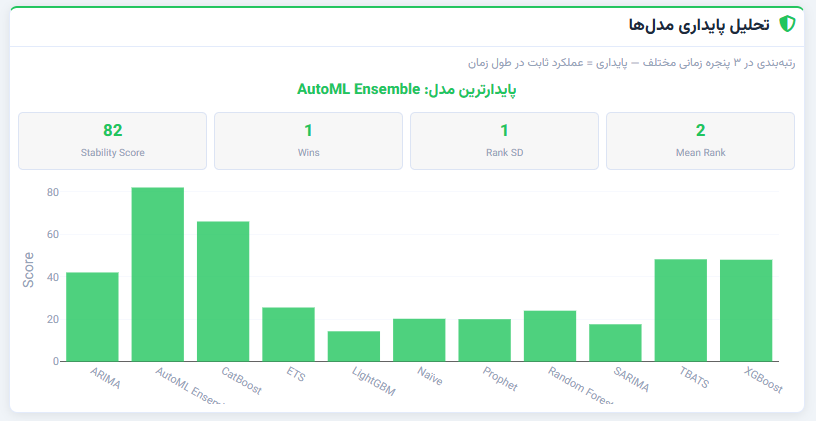
\includegraphics[width=0.6\linewidth]{figs/stability_analysis.png}
		\caption{خروجی واقعی سامانه برای تحلیل پایداری رتبه‌بندی مدل‌ها.}
	\end{figure}
	\FloatBarrier
	
	\subsection{معیارهای ارزیابی ریاضی}
	برای مقایسه ۱۱ مدل، سیستم به یک معیار واحد اتکا ندارد.
	\begin{itemize}
		\item \textbf{\lr{RMSE} (جذر میانگین مربعات خطا):}
		\begin{equation}
			RMSE = \sqrt{\frac{1}{n}\sum_{i=1}^{n} (y_i - \hat{y}_i)^2}
		\end{equation}
		\item \textbf{\lr{MAE} (میانگین قدر مطلق خطا):}
		\begin{equation}
			MAE = \frac{1}{n}\sum_{i=1}^{n} |y_i - \hat{y}_i|
		\end{equation}
		\item \textbf{$R^2$ (ضریب تعیین):} نشان می‌دهد که مدل ما چقدر توانسته واریانس داده‌ها را توضیح دهد.
	\end{itemize}
	
	% ==========================================================
	\section{تحلیل نتایج و شواهد}
	% ==========================================================
	پس از اجرای پایپ‌لاین کامل و ارزیابی ۱۱ مدل بر روی ۵ کلان‌شهر ایران، نتایج به دست آمده شواهد روشنی از نقاط قوت و ضعف الگوریتم‌های داده‌محور ارائه می‌دهد.
	
	\subsection{پارادوکس دقت در کوتاه‌مدت}
	یکی از شگفت‌انگیزترین نتایج بنچمارک ۲۴ ساعته، رقابت بسیار نزدیک مدل‌های پیچیده با ساده‌ترین مدل موجود، یعنی \textbf{\lr{Naïve}} بود.
	\begin{itemize}
		\item \textbf{دلیل علمی:} جرم هوا در یک منطقه در کوتاه‌مدت به سرعت تغییر نمی‌کند.
		\item \textbf{نتیجه:} مدل‌های \lr{ML} به سختی توانستند از مدل \lr{Naïve} پیشی بگیرند.
	\end{itemize}
	
	\begin{figure}[htbp]
		\centering
		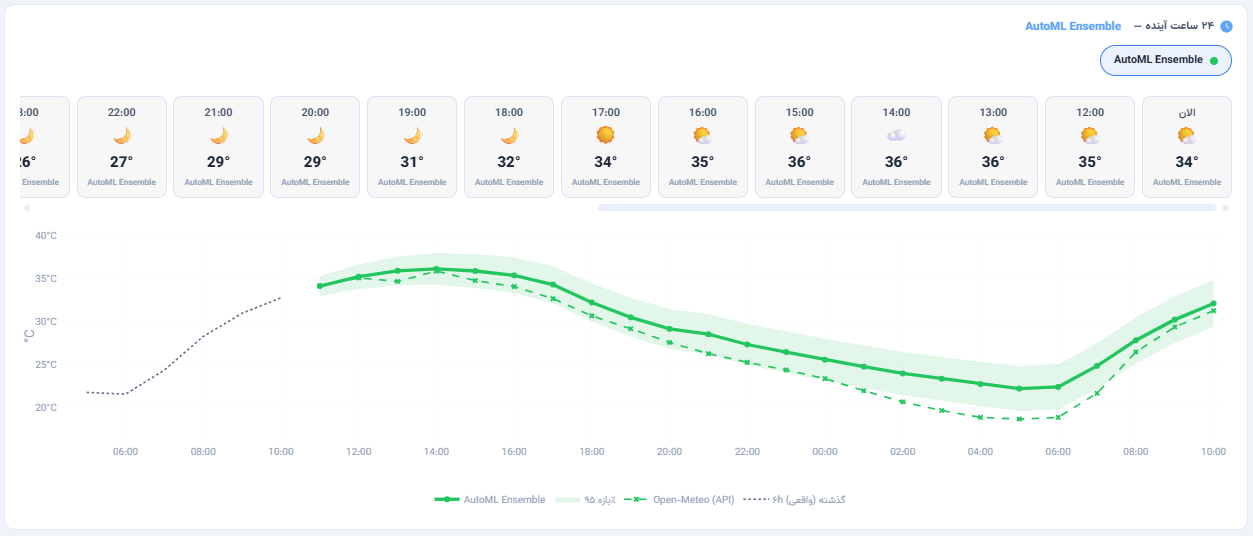
\includegraphics[width=0.85\linewidth]{figs/forecast_24h.png}
		\caption{نمای واقعی پیش‌بینی ۲۴ ساعته اصفهان در داشبورد}
	\end{figure}
	\FloatBarrier
	
	\subsection{مرز دقت مدل‌های داده‌محور و ضرورت مدل‌های \lr{NWP}}
	شواهد نشان داد:
	\begin{itemize}
		\item \textbf{افق ۱ تا ۳ روز:} مدل‌های داده‌محور کاملاً مستقل هستند و می‌توانند با دقت بالا ($R^2 > 0.90$) با مدل‌های \lr{NWP} رقابت کنند.
		\item \textbf{افق ۴ تا ۷ روز:} تغییرات جبهه‌های هوایی باعث می‌شود دقت \lr{ML} به شدت افت کند.
		\item \textbf{راه‌حل نهایی:} با میانگین‌گیری ۵۰-۵۰ بین خروجی \lr{ML} و \lr{Open-Meteo}، توانستیم یک پیش‌بینی پایدار تولید کنیم.
	\end{itemize}
	
	\begin{figure}[htbp]
		\centering
		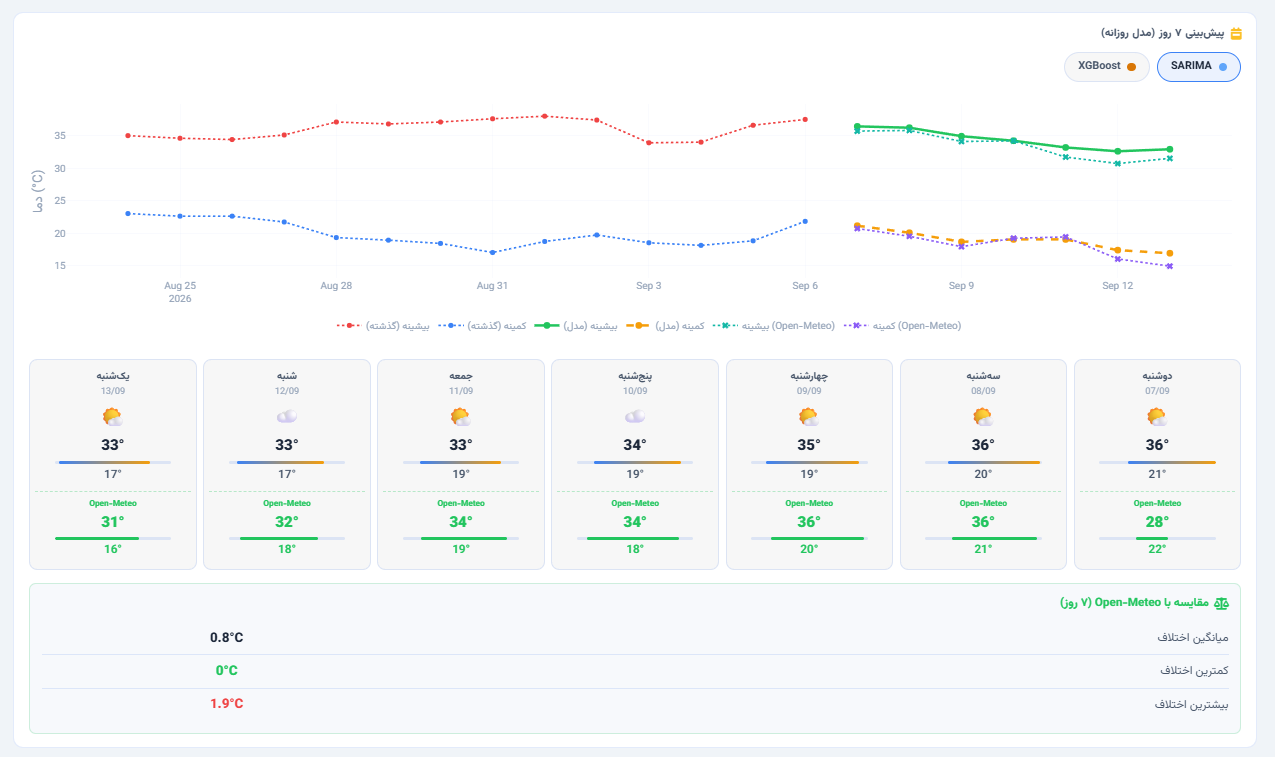
\includegraphics[width=0.85\linewidth]{figs/forecast_7day.png}
		\caption{پیش‌بینی ۷ روزه به تفکیک هر روز در داشبورد.}
	\end{figure}
	\FloatBarrier
	
	\vspace{1cm}
	\begin{center}
		\textbf{نتیجه‌گیری نهایی گزارش}
	\end{center}
	این پروژه نشان داد که یادگیری ماشین جایگزین مطلق فیزیک اتمسفری نیست؛ بلکه مکمل آن است.
	
	% ==========================================================
	\section{پیشنهادات و جهت‌گیری‌های آینده}
	% ==========================================================
	با توجه به یافته‌های این پژوهش، مسیرهای زیر پیشنهاد می‌شود:
	\begin{itemize}
		\item \textbf{بهره‌گیری از مدل‌های یادگیری عمیق:} افزودن معماری‌هایی مانند \lr{LSTM}.
		\item \textbf{وزن‌دهی پویا در موتور ترکیبی:} به‌روزرسانی وزن‌ها بر اساس عملکرد اخیر هر مدل.
		\item \textbf{پیش‌بینی احتمالاتی:} ارائه بازه‌های اطمینان به جای یک عدد قطعی.
	\end{itemize}
	
\end{document}